
\documentclass[12pt,a4paper,twoside,openright]{scrreprt}
\usepackage[utf8]{inputenc}
\usepackage[british]{babel}
\usepackage{geometry} % see geometry.pdf on how to lay out the page. There's lots.
\usepackage[usenames,dvipsnames,svgnames,table]{xcolor}
\usepackage{graphicx}
\usepackage{caption}
\usepackage{setspace}
\usepackage{enumerate}
\usepackage{adjustbox}
\usepackage{minted}
\usepackage{tabu}
\usepackage[T1]{fontenc}
\usepackage{amsmath}
\usepackage{ amssymb }
\usepackage{cutwin}
%\usepackage{bm}
\usepackage{url}
\usepackage{centernot}
\usepackage{mathtools}
\usepackage{cancel}
\usepackage{turnstile}
\usepackage{pdflscape}
\usepackage{tikz}
\usepackage{siunitx}
\usepackage[full]{textcomp}
\usepackage[osf]{newpxtext} % osf for text, not math
\usepackage{cabin} % sans serif
\usepackage[varqu,varl]{inconsolata} % sans serif typewriter
\usepackage[bigdelims,vvarbb]{newpxmath} % bb from STIX
\usepackage[cal=boondoxo]{mathalfa} % mathcal
\usepackage{hyperref}
\usepackage[style=ieee]{biblatex}
\usepackage[capitalise]{cleveref}


\usemintedstyle{tango}

\addbibresource{dissertation.bib}

\crefformat{section}{§#2#1#3}
\Crefformat{section}{§#2#1#3}

\crefrangeformat{section}{§§#3#1#4--#5#2#6}
\Crefrangeformat{section}{§§#3#1#4--#5#2#6}

\crefmultiformat{section}{§§#2#1#3}{ and~#2#1#3}{, #2#1#3}{ and~#2#1#3}
\Crefmultiformat{section}{§§#2#1#3}{ and~#2#1#3}{, #2#1#3}{ and~#2#1#3}

\crefrangemultiformat{section}{§§#3#1#4--#5#2#6}{ and~#3#1#4--#5#2#6}{, #3#1#4--#5#2#6}{ and~#3#1#4--#5#2#6}
\Crefrangemultiformat{section}{§§#3#1#4--#5#2#6}{ and~#3#1#4--#5#2#6}{, #3#1#4--#5#2#6}{ and~#3#1#4--#5#2#6}

\setlength{\oddsidemargin}{-0.4mm}    % 25 mm left margin - 1 in
\setlength{\evensidemargin}{\oddsidemargin}
\setlength{\topmargin}{-5.4mm}        % 20 mm top margin - 1 in
\setlength{\textwidth}{160mm}         % 20/25 mm right margin
\setlength{\textheight}{237mm}        % 20 mm bottom margin
\setlength{\headheight}{5mm}
\setlength{\headsep}{5mm}
\setlength{\parindent}{0mm}
\setlength{\parskip}{\medskipamount}
\renewcommand\baselinestretch{1.15} % thesis format (not needed for techreport)
% don't let large figures hijack entire pages
\renewcommand\topfraction{.9}
\renewcommand\textfraction{.1}
\renewcommand\floatpagefraction{.8}

\newcommand{\mlpos}{}

\newcommand{\exs}[1]{\mintinline{elixir}{#1}}

\newcommand{\todo}[1]{\fcolorbox{red}{white}{\parbox{0.9\textwidth}{\textbf{TODO:} {#1}}}}

\AtBeginEnvironment{minted}{%
  \renewcommand{\fcolorbox}[4][]{#4}}
  
\AtBeginEnvironment{mintinline}{%
  \renewcommand{\fcolorbox}[4][]{#4}}

\makeatletter
\DeclareFontFamily{OMX}{MnSymbolE}{}
\DeclareSymbolFont{MnLargeSymbols}{OMX}{MnSymbolE}{m}{n}
\SetSymbolFont{MnLargeSymbols}{bold}{OMX}{MnSymbolE}{b}{n}
\DeclareFontShape{OMX}{MnSymbolE}{m}{n}{
    <-6>  MnSymbolE5
   <6-7>  MnSymbolE6
   <7-8>  MnSymbolE7
   <8-9>  MnSymbolE8
   <9-10> MnSymbolE9
  <10-12> MnSymbolE10
  <12->   MnSymbolE12
}{}
\DeclareFontShape{OMX}{MnSymbolE}{b}{n}{
    <-6>  MnSymbolE-Bold5
   <6-7>  MnSymbolE-Bold6
   <7-8>  MnSymbolE-Bold7
   <8-9>  MnSymbolE-Bold8
   <9-10> MnSymbolE-Bold9
  <10-12> MnSymbolE-Bold10
  <12->   MnSymbolE-Bold12
}{}

\let\llangle\@undefined
\let\rrangle\@undefined
\DeclareMathDelimiter{\llangle}{\mathopen}%
                     {MnLargeSymbols}{'164}{MnLargeSymbols}{'164}
\DeclareMathDelimiter{\rrangle}{\mathclose}%
                     {MnLargeSymbols}{'171}{MnLargeSymbols}{'171}
\makeatother

\setcounter{tocdepth}{2}



%%% BEGIN DOCUMENT
\begin{document}


\begin{titlepage}
\rightline{\LARGE \textbf{Mateusz Jadczak}}

\vspace*{60mm}
\begin{center}
\Huge
\textbf{An implementation of Google Dataflow in the Elixir programming language} \\[5mm]
Computer Science Tripos -- Part II \\[5mm]
Robinson College \\[5mm]
XX May 2017
\end{center}
\end{titlepage}

% Proforma


{\let\cleardoublepage\clearpage \chapter*{Proforma}} % Start on next side

{\large
\begin{tabu}{ll}
Name:               & \textbf {Mateusz Jadczak}                       \\
College:            & \textbf {Robinson}                     \\
Project Title:      & \textbf {TODO MULTILINE} \\
Examination:        & \textbf {Computer Science Tripos -- Part II, June 2017}  \\
Word Count:         & XX\footnotemark[1]  \\
Project Originators: & Dr Alastair Beresford \& Dr Martin Kleppmann     \\
Supervisor:         &   Dr Alastair Beresford           \\ 
\end{tabu}
}
\footnotetext[1]{This word count was computed
using the \texttt{texcount} tool.
}
\stepcounter{footnote}

\bigskip

\section*{Original aims of the project}

TODO


\section*{Work completed}

TODO

\section*{Special difficulties}

TODO
\newpage
\section*{Declaration}

I, Mateusz Jadczak of Robinson College, being a candidate for Part II of the Computer
Science Tripos, hereby declare
that this dissertation and the work described in it are my own work,
unaided except as may be specified below, and that the dissertation
does not contain material that has already been used to any substantial
extent for a comparable purpose.

\bigskip
\leftline{Signed}

\medskip
\leftline{Date}


%\tableofcontents

%\listoffigures

%\newpage


\chapter{Introduction}\label{ch:intro}

\section{Background}\label{sec:intro:background}

In today's fast-moving world of technology, data is king.
The ability to quickly and flexibly process large, heterogeneous and asynchronous streams of data, is core to many businesses, and this need is only increasing \cite{Yin_2015}\cite{mit_bean_variety}.

Of particular interest are datasets which are inherently unordered and unbounded.
For instance, consider the issue of tracking listen counts of songs on a service like Spotify, where some views may occur on cached data stored offline, and may not be sent to the servers until hours later.
Even more trivially, when operating at a global scale, simple issues like clock skew and network latency mean that we cannot expect data to arrive in-order.

Now, suppose we need to aggregate the track listen events into user sessions, defined as listen events occurring sufficiently close to each other.
The amount of complexity and number of special cases even in this reasonable scenario are too large to consider its implementation with dedicated logic.
There is a clear need for an underlying data model and abstraction in order to sanely manage this kind of processing.

Solutions to this problem have been proposed and implemented in open-source systems such as Apache Storm \cite{apache_storm} and Spark Streaming \cite{spark:zaharia2013discretized}, as well as internally in projects like Google's MillWheel \cite{akidau2013millwheel}.
These projects focus on the concept of \emph{stream processing}---the assumption that the inputs are (possibly unbounded, or never-ending) streams of data.
They apply techniques such as windowing, triggering and watermark tracking to make processing this kind of data possible, but in general fall short on sundry features like scalability and fault tolerance, correctness, expressiveness, richness of windowing features, and others.
The key insight is that these solutions are narrowly scoped for particular problem domains, instead of taking a general approach.

\section{Motivation for the Dataflow Model}\label{sec:intro:motivation}

The issues set out in the previous section drove the development of a new, unified model of data processing at Google ~\cite{Akidau:2015}.
This section simply aims to set out the core motivation behind the model, answering the question, ``Why do we need yet another core tool?''

\begin{figure*}[h]
	\centering
	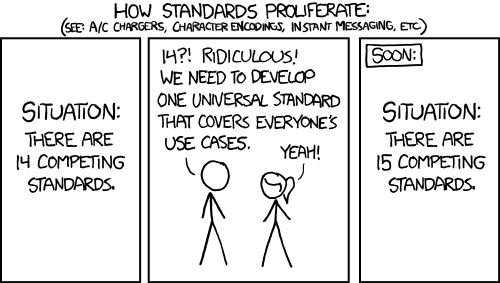
\includegraphics[width=.75\textwidth]{images/xkcd-standards}
	\caption*{\textit{Source: https://xkcd.com/927/\quad(CC BY-NC 2.5)}}
\end{figure*}

Simply put, the Dataflow Model aims to provide a unified way of thinking about data processing, producing a clear, composable abstraction.
It acknowledges the fact that it is impossible to design a perfect (always correct, low-latency and cheap) system, and instead it allows for tunability across these characteristics.

\Cref{sec:prep:dataflow} dives deep into the model itself and explains how these aims are achieved, while \cref{ch:impl} contains a detailed overview of the implementation of the model in practice.

\section{Why Elixir?}\label{sec:intro:elixir}

The Elixir language \cite{Elixir} is relatively young.
It is currently most popular in the web development circles, with many treating it as a Ruby replacement.
How then is this a suitable language in which to implement a robust, complex data processing system?

The answer lies in the underpinnings of the language.
Beneath the shiny, modern exterior lies the battle-hardened BEAM VM and OTP framework, which have been running Erlang-powered systems, mostly in the telecommunications industry, for decades.
We also have at our disposal the entire ecosystem of libraries written for Erlang.

Elixir is a dynamically typed, functional language with no variable mutability and with built-in support for efficiently managing and scheduling hundreds of thousands of \emph{processes} (akin to greenthreads) in a manner which is similar to the Calculus of Sequential Processes.
This invites the use of an actor-based model for applications, and indeed this is the standard approach in the Elixir/BEAM ecosystem.
These built-in primitives allow us to closely implement the desired semantics of the Dataflow Model without the overhead of thousands of lines of scheduling, threading and co\"ordinating\footnotemark[1] code (present in the existing Java implementation).

\footnotetext[1]{
For the typographically observant reader: the \"{} mark in ``co\"ordinating'' is a diaeresis---one of the two diacritical marks which are part of English natively (the other being the grave, as in ``the learn\`ed scholar'').
While its use is uncommon in modern English, some publications (notably The New Yorker) still employ it, and including it is the preferred style of the author.
It is used to indicate that two vowels should be pronounced separately, and not as a diphthong.
}

This project was completed using Elixir v1.4.2, and so all code examples and statements about the language apply to this version, the most current at the time of writing.
\Cref{sec:prep:elixir} gives a brief introduction to the language.



\section{Previous work}\label{sec:intro:previous}
Since the publication of the Dataflow paper \cite{Akidau:2015}, work has been ongoing to implement the Model in practice.
Initially, Google released the Google Cloud Dataflow product \cite{CloudDataflow} along with an SDK to allow users to easily construct data processing pipelines and run them on Google's cloud infrastructure.

In early 2016, Google decided to open-source the project and place it under the care of the Apache Foundation \cite{ApacheDataflowPost}.
This marked the beginning of Apache Beam, a project whose goals were even wider, and include support for cross-platform, cross-language compatibility through separating the creation of the pipelines and their execution on \emph{runners}.

The project has made excellent progress on these fronts, with a fully-featured SDK written in Java as well as a Python SDK.
It is compatible with many data processing systems such as Apache projects Spark, Storm and Flink.
Google Cloud Dataflow remains a paid product capable of running Beam pipelines at scale, but is now only one of many options for doing so.

The implementation also includes an on-machine local runner mainly aimed at testing workflows.
As the simplest yet fully-featured implementation of a Beam runner, it was used as the reference implementation for this project.

Several of the concepts introduced in the Dataflow paper have been used in other projects.
Notably, in the Elixir ecosystem, the Flow project \cite{ElixirFlow} takes some of the concepts---such as the windowing and triggering model---and provides a highly idiomatic way to write and execute multi-threaded computation in Elixir.
Its goals are, however, much narrower than the full Dataflow Model.

Flow has driven the development of GenStage \cite{ElixirGenStage}, a more low-level library implementing demand-driven data flow between actor processes, along with an extensible way to route, partition and dispatch that data.
GenStage forms the backbone of the execution logic in this project, and it is described in more detail in \cref{sec:todo}.

\section{Terminology}\label{sec:intro:terminology}

There are several similar and overloaded terms employed in this dissertation.
This section aims to clarify these and set a convention to be followed.
For a full list of defined terms, the reader should consult the <ref here to Appendix: Glossary>.

Due to the naming change to Apache Beam on open-sourcing the project, the reader will find various references to both the ``Dataflow`` and ``Beam`` on the web with little consistency.

The approach taken in this paper is to refer to the theoretical model described in \cite{Akidau:2015} as the Dataflow Model, and to the current, de facto official, implementation \cite{ApacheBeam} as Beam (generally referred to in full as Apache Beam).
Further, where the ``Beam Model'' is referenced, the author means the Dataflow extended with concepts now found in Apache Beam.
An overview of these is found in \cref{sec:impl:dataflow}.

The virtual machine which powers Erlang and Elixir is called the BEAM.
While efforts are made to refer to the conflicting software in full as the BEAM VM and Apache Beam, the reader should note that wherever the virtual machine is referred to, BEAM appears in all-uppercase form.

\section{Goals and focus}\label{sec:intro:goals}

At the outset, the goal of the project was to write an Elixir-based SDK in order to create Pipelines which could run on the existing Beam software.
Several weeks into the research it emerged concurrently that this approach was impractical to achieve, and that the front-end DSL itself was a relatively small task in itself, not suitable to form the entirety of the project.

The goal then shifted to writing an implementation of a subset of the Beam Model in Elixir.
However, due to the lack of explicit technical documentation of the Model, very quickly it emerged that in order to do this, a very significant amount of work had to be done to reverse-engineer it from an existing open-source codebase and community discussions.
As explained in \cref{sec:impl:dataflow}, many concepts have to be introduced in order to implement the Model, but they are not described directly in any reference material.

Therefore, a second goal of the project emerged, which proved to be a major focus---to extend and clarify the Dataflow Model with the concepts found in Apache Beam, such that a fuller, implementation-ready description is produced.
Once this work was completed, the initial goal of implementing this extended model was achieved with some additional effort.

\section{Results achieved}

Overall, the project was a success, in spite of proving much more challenging than originally imagined.
Due to the highly uncertain nature of the requirements, code had to be continually revisited and improved upon, and evaluation of progress was not straightforward.

Nevertheless, a working implementation of the Model was produced.
The implementation, while forgoing some features, delivered robust performance and a clean programmer interface, meshing well with existing language conventions.

A significant amount of currently non-existent documentation of the theory of the Beam Model was also produced, with some further extensions introduced which solve problems currently being tackled in the Beam Project.



\chapter{Preparation}\label{ch:prep}

\section{The Elixir programming language (a primer)}\label{sec:prep:elixir}

\subsection{Language basics}

\subsection{Concurrency model and the OTP framework}

\section{The Dataflow Model explained}\label{sec:prep:dataflow}

As mentioned in \cref{sec:intro:motivation}, the main feature of the Dataflow model is flexibility.
It aims to create a unified model of data processing which can encompass other processes, placing them in a well-defined structure and allowing the efficient execution of such systems.

It does this by separating the logical notion of data processing from the underlying physical implementation.
An abstract data processing model is defined which covers existing modes of processing by allowing the orthogonal specification of \textbf{what} results are being computed, \textbf{where} in event time they are being computed, \textbf{when} in processing time they are materialised, and \textbf{how} earlier results relate to later refinements \cite[p.~1793]{Akidau:2015}.

This standard model can then be implemented and realised by many different runners, whether natively batch, streaming or hybrid, each with its own set of advantages and disadvantages. 
This flexible approach allows for the tuning of execution technology to business requirements while working with a consistent, expressive theoretical model of the processing itself.

The key takeaway is that this model tries to make as few assumptions as possible on the data inputs, outputs and processes, instead providing simple primitives from which complex system can be constructed.

What follows is a descriptions of the primitive concepts used in the model to more precisely specify all of these properties.

\subsection{``The What'': Transforms and pipelines}\label{sec:prep:dataflow:what}

In the Dataflow model, a \emph{pipeline} is an entire data processing flow.
It may incorporate many different \emph{transforms} which pass data between each other, processing and transforming it as it flows through them.
One can think of pipelines as DAGs\footnote{Directed Acyclic Graphs}, with nodes representing transforms and edges representing the data flowing between them.

\todo{Diagrams of pipelines}

The graph does not have to be connected---it is valid for there to be multiple disjoint data processing paths.
A given transform may produce multiple outputs and it may take in multiple inputs.
It can also produce no outputs, instead causing a side effect such as writing to the network, database or file system.
Transforms can also have no inputs in the graph, instead receiving output from an external source or generating it.
These transforms are called root transforms.

A key advantage of expressing transforms in terms of data flowing is the natural adaptation of the system to unbounded data.
When we say unbounded data, we mean data which may not necessarily have an end.
An example of this may be a stream of events from a website, or the Twitter firehose.
It may help to think of unbounded data as ``streaming'' data, but ``streaming'' and ''batch'' imply execution strategies as opposed to data properties.
Further, in the Dataflow Model it is more convenient to think of all data as being streamed, whether that is a true infinite stream, or merely data being streamed out of a file.

All transforms can be represented fundamentally using only two primitives: \verb|ParDo| and \verb|GroupByKey|\footnotemark[2].

\footnotetext[2]{
Even though these transforms are the only primitives mentioned in the original description of the Model \cite[§2.1]{Akidau:2015}, real implementation will likely special-case several other transforms such as \texttt{AssignTimestamps} or \texttt{Window} and make them primitives for architectural or performance reasons.
}

\todo{diagrams of the transformations performed by these}

\verb|ParDo| represents a flat-map operation---it transforms a data element into zero or more data elements.
The actual computation performed can be arbitrary---the only restriction is that the output depends only on the single element being processed.
This restriction means that the \verb|ParDo| step is ``embarrassingly parallelisable''.
It also translates naturally to operating on unbounded data, as we can emit the output in real-time.

\verb|GroupByKey|, on the other hand, simply groups all key-value pairs into elements with a single key and a collection of elements.
It needs to collect \emph{all} of the data for a particular key before being able to emit its output.
An issue arises when dealing with unbounded data---how do we know when we've received all of the input for a particular key?

To deal with this problem, the Dataflow Model introduces a concept of windowing.

\todo{somewhere we need an explanation of elements' structure as they flow through the pipeline.}

\subsection{``The Where'': Windowing}\label{sec:prep:dataflow:where}

Windowing simply means the additional grouping of elements according to their timestamps in a way which allows us to emit a particular chunk of elements when we know that we have all the data for it.
In the Dataflow Model, we call such a chunk of data belonging to a particular window a \emph{pane}.
Before diving into the details, let us take a brief detour into what ``time'' means in this context.

\subsubsection{Time domains}
We distinguish between two inherent time domains when considering our data as events in time: \emph{event time} and \emph{processing time}.

Event time is the time at which the event actually occurred and is an inherent property of the element itself.
We also refer to this value as the \emph{timestamp} of an element.
Each element in a pipeline must have a timestamp.
We ensure that we have two ``special'' values available, the \emph{minimum} and \emph{maximum timestamps}.
Implementations may make these actual special values, or just use the maximal and minimal values of the underlying representation.

Where there is no inherent time associated with an element (for example it is an un-dated record in a file) or we don't know the timestamp yet (we must process the record before we can extract the timestamp), the element is assigned the minimum timestamp.
The logic of this will become apparent in the following sections.

Processing time is the property of an executing pipeline.
It measures real-world time elapsing as the computation progresses.
The processing time of a particular element at a particular transform is simply the system clock time at which it was seen or processed by that transform.
The Model makes no assumptions about the synchronisation of this time across multiple distributed transforms.

\subsubsection{Types of windows}

\todo{describe global, fixed, sliding and session windowing}

\todo{diagrams showing visually how different windows work}

\subsubsection{Windowing in the Dataflow Model}
The key insight in the Dataflow Model which allows for very flexible windowing is the generalisation of what a window is.

We define the concept of a \emph{windowing function}, which is actually a pair of two functions: \texttt{assign} and \texttt{merge}.

\texttt{assign} takes the timestamp of the element (and optionally the element's data) and outputs a set of windows to which it should be assigned.
This may be a singleton set when windows are non-overlapping, or it could be many windows in the case of e.g.\ sliding windows.
It's important to note that if the element is assigned to multiple windows, we are essentially duplicating that element into each of those windows (since all computation is implicitly grouped by the window).

\texttt{merge} takes a set of windows and optionally merges some or all of them into a new set of windows.
This is used in windowing strategies such as the session windowing mentioned earlier---this function will detect smaller windows near each other and merge them into longer sessions.
Not all windowing functions take advantage of this, and in fact the common strategies apart from session windows are all non-merging.

\todo{diagram / example of how values are transformed with windowing and grouping}

\todo{show an example of the two functions being used to effect session-based windowing}

\subsection{``The When'': Watermarks and triggers}\label{sec:prep:dataflow:when}

In the previous section, we have defined a way to group elements together into windows.
We have also asserted that we can ``emit a particular chunk of elements when we know that we have all the data for it''.
How can we achieve this in light of the fact that data may appear out of order?

The true answer is that we cannot---if we allow the possibility of unpredictably late data in our pipeline, then we cannot ever truly be certain that we can emit a complete pane of data.
What we can do, however, is introduce a model which allows us to specify the desired behaviour in a useful and flexible manner.
Let us first define the concept of \emph{watermarks}.

\subsubsection{Watermarks}

A \emph{watermark} is a lower bound, in event time, on the timestamps of values which have been processed by the pipeline (or a particular transform therein).
For example, if at a particular instant the watermark is time $T$, then we are being promised that all events with timestamps earlier than $T$ have been processed.
A graph of watermark progression against processing time (such as the one in <TODO ref here>) is a useful way to visualise the progress of a pipeline.
Further, this concept allows us to construct a powerful model of lateness in the system.
This is explored further in \cref{sec:prep:dataflow_extra:lateness}.

\todo{diagram of elements being processed in time vs.\ a watermark}

The reader may at this point be asking, ``where does the watermark come from?''
Watermarks in the Dataflow Model are heuristics generated by sources of data, or by user logic in the pipeline.
The exact behaviour is described in \cref{sec:impl:dataflow}.

\subsubsection{Triggering model}

An initial suggestion may be to simply use the watermark as an indication of when a window is finished and is safe to emit; that is, to emit once the watermark has passed the end of the window.
There are two major shortcomings with this strategy:
\begin{itemize}
	\item The watermark may be \textbf{too fast}---we may have decided that all elements for a given window have been seen and emit a pane, only to later on receive a late element which should have been in the window.
	It is unclear what to do with the element in this case.
	
	\item The watermark may be \textbf{too slow}---the heuristic can be too conservative, and even when we have access to the true watermark and not merely a heuristic, a single slow datum can hold up processing for the entire pipeline.
	Therefore using watermarks as the sole signal for emitting data can lead to high latency which may be highly undesirable in some scenarios.
\end{itemize} 

To solve these problems, we define a more complex triggering model.

Firstly, we explicitly allow for data in a particular window to be emitted multiple times.
We call each such emission a pane, and every pane is marked as either early, on time or late.
Secondly, we define a trigger as simply some arbitrary code which has access to time information of elements passing through the transform, as well as watermark and other timing information.
In practice, we define a tree of triggers allowing us to easily achieve desired results (this is explored further in <todo ref>). 

In this manner we can allow for many different behaviours---for example, we may want to receive approximate results (early panes) every ten seconds (in processing time) until the watermark passes the end of the window, at which point an on time pane is emitted.
Any further late data arriving after the watermark can trigger the emission of a late pane.
This, and myriad other combinations, are all possible with this model.
A key strength is that it decouples the marking of data as early/tentative, on time/definitive, or late/corrective, from actually processing the different panes in different ways.

\todo{maybe include a description of a particular use case and which options one would choose for it?}

\todo{one sentence conclusion of triggering / windowing}

\subsection{``The How'': Refinements and retractions}\label{sec:prep:dataflow:how}

While the concepts defined so far allow us to specify when panes should be emitted, we haven't yet settled on what their contents should be, exactly.
We do this by selecting from one of the three refinement modes for a particular \verb|GroupByKey| transform:
\begin{itemize}
	\item The \textbf{discarding} mode simply discards the contents of the window after emitting a pane, such that any new pane emitted will contain only data received since the last emission. There is no relation between the contents of any two panes.
	\item The \textbf{accumulating} mode retains the contents of the window after emitting a pane. A later pane will include all of the data from the initial pane, in addition to any data which has arrived since.
	\item The \textbf{accumulating \& retracting} mode emits retractions to previous panes emitted, as well as following the semantics of the accumulating mode. This means that downstream transforms will first receive notification that the previous pane is now invalid (along with the contents of that pane again, to aid in undoing its results), and after this they will receive the contents of the new pane (which includes the contents of the initial pane, now refined with additional data). 
\end{itemize}

\todo{example of when to use one or the other?}

While the Model broadly defines the concept of retractions and how they may work at a high level, their implementation remains an unsolved problem and is actively being worked on by the Beam project.
The main difficulty lies in the explosion of cached state which seems to be needed in order to allow the undoing of certain operations.
Therefore, the implementation and precise specification of the behaviour of retractions are out of the scope of this paper, and will not be mentioned again.

With the core primitives of the Dataflow Model defined, we will now briefly look at the work done in extending it into a production-ready implementation by the Apache Beam project before considering the additional theory and concepts which must be defined in order to specify the behaviour of such an implementation.

\section{A survey of the Apache Beam project}\label{sec:prep:beam}

The Apache Beam project is a multifaceted undertaking, aiming to build an entire ecosystem around the Model.
The components of the project can be coarsely categorised into SDKs and \emph{runners}.

SDKs provide the user interface to the processing engine.
They are language-specific libraries which allow users to specify the computations to be performed using the tools of their native language, without having to worry about how the computation will be executed.
Currently there is a main, fully-featured Java SDK which serves as the \emph{de~facto} standard implementation.
There is also work being done on a Python version of the SDK.

\todo{``as of the time of writing''?}

SDKs produce descriptions of data processing pipelines in a standard format, which any runner can consume and execute.
This allows the flexibility of being able to select and tune the execution engine orthogonally to the computation itself in accordance with the needs of each user, while keeping a lot of this complexity out of the user-facing data processing model.

As mentioned in \cref{sec:intro:previous}, there is a commercial runner available through Google's Cloud Dataflow product \cite{CloudDataflow} which is a fully-managed, auto-scaling service to execute Beam pipelines.
There are also many runners which utilise other open-source data processing projects, helping to leverage existing resources or run large workloads on-premises rather than in the cloud.

Not all runners support all of the model's features, and the range of support is summarised in \emph{capability matrices}.
A full copy of the official capability matrix can be found in <appendix ref>.

\todo{larger question: is it worth referencing JIRA issues or mailing list discussions? Is it ok to just assert that certain things are the case or are being worked on?}

\todo{include capability matrices? Maybe construct one for this implementation? (https://beam.apache.org/documentation/runners/capability-matrix/)}

A crucial part of the Beam project is the \verb|DirectRunner|---the local on-machine runner provided with the Java SDK.
Its aims are not to necessarily provide a high-performance implementation, but rather to act as the standard implementation of behaviour for other runners to follow.
It is used by users to test out pipelines before sending them to a large-scale runner for production-scale execution.
In fact, much of its functionality is in a separate ``Core'' module, which contains code for other runners to directly use.

This runner is crucial for this project, as it is the result of many man-years of work to come up with a practical implementation of the Dataflow Model while keeping with its definition.
It is the runner whose main focus is model correctness, and as such it is the most appropriate to take as a reference implementation for a project which aims to explore the Dataflow Model, such as this one.


\section{Changing goals}

A side-effect of the way the Dataflow/Beam project has developed is that a large amount of development of the theory of the model has occurred implicitly while the software was worked on.
This happened in place of a formal definition of many concepts, a large amount of which were sketched out in proposals for the project and then iterated upon in code.

Therefore, a huge part of this project was the extraction and reverse-engineering of these concepts from the Java codebase into a more formal specification.
This was further necessitated by the move from an OOP to a functional approach, requiring each concept to be reduced to what it is in the abstract rather than just transferring the class hierarchy to a new language.

The initial project goals did not account for this---it was assumed that a reasonable implementation could be produced from the Dataflow paper \cite{Akidau:2015} using the Beam code simply as reference.


\section{Software Engineering methods}\label{sec:prep:softeng}

\subsection{The spiral model}


This resulted in a need for a highly adaptive and agile development process, since fundamental assumptions made initially changed many times over.

\todo{give actual examples of this happening maybe?}

The Elixir language, with its clear modular structure combined with writing simple, composable functions enabled a flexible model where key logic in the codebase could be refactored with ease when needed.

\todo{summarise spiral model, refer to previous subsection as to why it's good. Include a diagram.}

\subsection{Testing approach}

\todo{mention small, testable modules as well as end-to-end examples}

\section{Starting point}\label{sec:prep:starting}

\todo{Good knowledge of Elixir, and not much more regarding getting to know how Beam ticks inside.}

\section{Summary}\label{sec:prep:summary}

\printbibliography

% Main document




\end{document}